\documentclass{ximera}

%\usepackage{todonotes}

\newcommand{\todo}{}

\usepackage{tkz-euclide}
\tikzset{>=stealth} %% cool arrow head
\tikzset{shorten <>/.style={ shorten >=#1, shorten <=#1 } } %% allows shorter vectors

\usepackage{tkz-tab}  %% sign charts
\usetikzlibrary{decorations.pathreplacing} 

\usetikzlibrary{backgrounds} %% for boxes around graphs
\usetikzlibrary{shapes,positioning}  %% Clouds and stars
\usetikzlibrary{matrix} %% for matrix
\usepgfplotslibrary{polar} %% for polar plots
\usetkzobj{all}
\usepackage[makeroom]{cancel} %% for strike outs
%\usepackage{mathtools} %% for pretty underbrace % Breaks Ximera
\usepackage{multicol}

\usepackage{polynom}



\usepackage[many]{tcolorbox}  %% for titled boxes
\newtcolorbox{xbox}[1]{%
    tikznode boxed title,
    enhanced,
    arc=0mm,
    interior style={white},
    attach boxed title to top center= {yshift=-\tcboxedtitleheight/2},
    fonttitle=\bfseries,
    colbacktitle=white,coltitle=black,
    boxed title style={size=normal,colframe=white,boxrule=0pt},
    title={#1}}


\usepackage{array}
\setlength{\extrarowheight}{+.1cm}   
\newdimen\digitwidth
\settowidth\digitwidth{9}
\def\divrule#1#2{
\noalign{\moveright#1\digitwidth
\vbox{\hrule width#2\digitwidth}}}





\newcommand{\RR}{\mathbb R}
\newcommand{\R}{\mathbb R}
\newcommand{\N}{\mathbb N}
\newcommand{\Z}{\mathbb Z}

%\renewcommand{\d}{\,d\!}
\renewcommand{\d}{\mathop{}\!d}
\newcommand{\dd}[2][]{\frac{\d #1}{\d #2}}
\newcommand{\pp}[2][]{\frac{\partial #1}{\partial #2}}
\renewcommand{\l}{\ell}
\newcommand{\ddx}{\frac{d}{\d x}}
\newcommand{\ddt}{\frac{d}{\d t}}

\newcommand{\zeroOverZero}{\ensuremath{\boldsymbol{\tfrac{0}{0}}}}
\newcommand{\inftyOverInfty}{\ensuremath{\boldsymbol{\tfrac{\infty}{\infty}}}}
\newcommand{\zeroOverInfty}{\ensuremath{\boldsymbol{\tfrac{0}{\infty}}}}
\newcommand{\zeroTimesInfty}{\ensuremath{\small\boldsymbol{0\cdot \infty}}}
\newcommand{\inftyMinusInfty}{\ensuremath{\small\boldsymbol{\infty - \infty}}}
\newcommand{\oneToInfty}{\ensuremath{\boldsymbol{1^\infty}}}
\newcommand{\zeroToZero}{\ensuremath{\boldsymbol{0^0}}}
\newcommand{\inftyToZero}{\ensuremath{\boldsymbol{\infty^0}}}



\newcommand{\numOverZero}{\ensuremath{\boldsymbol{\tfrac{\#}{0}}}}
\newcommand{\dfn}{\textbf}
%\newcommand{\unit}{\,\mathrm}
\newcommand{\unit}{\mathop{}\!\mathrm}
\newcommand{\eval}[1]{\bigg[ #1 \bigg]}
\newcommand{\seq}[1]{\left( #1 \right)}
\renewcommand{\epsilon}{\varepsilon}
\renewcommand{\iff}{\Leftrightarrow}

\DeclareMathOperator{\arccot}{arccot}
\DeclareMathOperator{\arcsec}{arcsec}
\DeclareMathOperator{\arccsc}{arccsc}
\DeclareMathOperator{\si}{Si}
\DeclareMathOperator{\proj}{proj}
\DeclareMathOperator{\scal}{scal}


\newcommand{\tightoverset}[2]{% for arrow vec
  \mathop{#2}\limits^{\vbox to -.5ex{\kern-0.75ex\hbox{$#1$}\vss}}}
\newcommand{\arrowvec}[1]{\tightoverset{\scriptstyle\rightharpoonup}{#1}}
\renewcommand{\vec}{\mathbf}
\newcommand{\veci}{\vec{i}}
\newcommand{\vecj}{\vec{j}}
\newcommand{\veck}{\vec{k}}
\newcommand{\vecl}{\boldsymbol{\l}}

\newcommand{\dotp}{\bullet}
\newcommand{\cross}{\boldsymbol\times}
\newcommand{\grad}{\boldsymbol\nabla}
\newcommand{\divergence}{\grad\dotp}
\newcommand{\curl}{\grad\cross}
%\DeclareMathOperator{\divergence}{divergence}
%\DeclareMathOperator{\curl}[1]{\grad\cross #1}


\colorlet{textColor}{black} 
\colorlet{background}{white}
\colorlet{penColor}{blue!50!black} % Color of a curve in a plot
\colorlet{penColor2}{red!50!black}% Color of a curve in a plot
\colorlet{penColor3}{red!50!blue} % Color of a curve in a plot
\colorlet{penColor4}{green!50!black} % Color of a curve in a plot
\colorlet{penColor5}{orange!80!black} % Color of a curve in a plot
\colorlet{fill1}{penColor!20} % Color of fill in a plot
\colorlet{fill2}{penColor2!20} % Color of fill in a plot
\colorlet{fillp}{fill1} % Color of positive area
\colorlet{filln}{penColor2!20} % Color of negative area
\colorlet{fill3}{penColor3!20} % Fill
\colorlet{fill4}{penColor4!20} % Fill
\colorlet{fill5}{penColor5!20} % Fill
\colorlet{gridColor}{gray!50} % Color of grid in a plot

\newcommand{\surfaceColor}{violet}
\newcommand{\surfaceColorTwo}{redyellow}
\newcommand{\sliceColor}{greenyellow}




\pgfmathdeclarefunction{gauss}{2}{% gives gaussian
  \pgfmathparse{1/(#2*sqrt(2*pi))*exp(-((x-#1)^2)/(2*#2^2))}%
}


%%%%%%%%%%%%%
%% Vectors
%%%%%%%%%%%%%

%% Simple horiz vectors
\renewcommand{\vector}[1]{\left\langle #1\right\rangle}


%% %% Complex Horiz Vectors with angle brackets
%% \makeatletter
%% \renewcommand{\vector}[2][ , ]{\left\langle%
%%   \def\nextitem{\def\nextitem{#1}}%
%%   \@for \el:=#2\do{\nextitem\el}\right\rangle%
%% }
%% \makeatother

%% %% Vertical Vectors
%% \def\vector#1{\begin{bmatrix}\vecListA#1,,\end{bmatrix}}
%% \def\vecListA#1,{\if,#1,\else #1\cr \expandafter \vecListA \fi}

%%%%%%%%%%%%%
%% End of vectors
%%%%%%%%%%%%%

%\newcommand{\fullwidth}{}
%\newcommand{\normalwidth}{}



%% makes a snazzy t-chart for evaluating functions
%\newenvironment{tchart}{\rowcolors{2}{}{background!90!textColor}\array}{\endarray}

%%This is to help with formatting on future title pages.
\newenvironment{sectionOutcomes}{}{} 



%% Flowchart stuff
%\tikzstyle{startstop} = [rectangle, rounded corners, minimum width=3cm, minimum height=1cm,text centered, draw=black]
%\tikzstyle{question} = [rectangle, minimum width=3cm, minimum height=1cm, text centered, draw=black]
%\tikzstyle{decision} = [trapezium, trapezium left angle=70, trapezium right angle=110, minimum width=3cm, minimum height=1cm, text centered, draw=black]
%\tikzstyle{question} = [rectangle, rounded corners, minimum width=3cm, minimum height=1cm,text centered, draw=black]
%\tikzstyle{process} = [rectangle, minimum width=3cm, minimum height=1cm, text centered, draw=black]
%\tikzstyle{decision} = [trapezium, trapezium left angle=70, trapezium right angle=110, minimum width=3cm, minimum height=1cm, text centered, draw=black]


\outcome{Understand the derivative as a function related to the original
  definition of a function.}
\outcome{Find the derivative function using the limit definition.}
\outcome{Relate the derivative function to the derivative at a point.}
\outcome{Relate the graph of the function to the graph of its derivative.}




\title[Dig-in:]{The derivative as a function}

\begin{document}
\begin{abstract}
Here we study the derivative of a function, as a function, in its own
right.
\end{abstract}
\maketitle

\section{The derivative of a function, as a function}


We know that to find the derivative of a function at a point $x=a$ we
write
\[
f'(a) = \lim_{h\to 0}\frac{f(a+h)-f(a)}{h},
\]
(provided that the limit exists).
However, if we replace the given number $a$ with a variable $x$, we now
have
\[
f'(x) = \lim_{h\to 0}\frac{f(x+h)-f(x)}{h},
\]
(provided that the limit exists).
This defines a new function $f'$, the derivative of $f$. The domain of $f'$ consists of all points in the domain of $f$ where the function $f$ is differentiable.
$f'(x)$ gives us the instantaneous rate of change of $f$ at any point $x$ in the domain of $f'$.\\
\begin{warning}
  The notation:
  \begin{quote}
  $f'(a)$ means take the derivative of $f$ first, then evaluate at
    $x=a$.
  \end{quote}
  In other words, given $f$ a function of $x$
  \[
  f'(a) = \eval{\ddx f(x)}_{x=a}.
  \]
\end{warning}
Given a function $f$ from the real numbers to the real numbers, the
derivative $f'$ is also a function from the real numbers to the real
numbers. Understanding the relationship between the \textit{functions}
$f$ and $f'$ helps us understand any situation (real or imagined)
involving changing values. 

\begin{question}
  Let $f(x) = 3x+2$. What is $f'(-1)$?
  \begin{multipleChoice}
    \choice{$f'(-1) = 0$ because $f'(3)$ is a number, and a number corresponds to a horizontal line, which has a slope of zero.}
    \choice[correct]{$f'(-1) = 3$ because $y=f(x)$ is a line with slope $3$.}
    \choice{We cannot solve this problem yet.}
  \end{multipleChoice}
\end{question}
\begin{example}
	Given the function $f(x) = 3x+2$, find  $f'(x)$. \\
	Then, use this this result to compute $f'(-1)$ in order to verify your answer in previous question.
	\begin{explanation}
		Start with the definition of $f'(x)$
		\[
		f'(x) = \lim_{h\to0}\frac{f(x+h)-f(\answer[given]{x})}{h}.
		\]
		Replace $f$ with its formula,
		\[
		f'(x) = \lim_{h\to0}\frac{3(x+h)+2-\answer[given]{(3x+2)}}{h}.
		\]
		Simplify the top,
		\[
		f'(x) = \lim_{h\to0}\frac{3\answer[given]{h}}{h}.
		\]
				Cancel the $h$ in the numerator and denominator,
		\[
		f'(x) = \lim_{h\to0}\answer[given]{3}.
		\]

		Evaluate the limit.
		\[
		f'(x) = \answer[given]{3}.
		\]
		Therefore,
		\[
		f'(-1) = \answer[given]{3}.
		\]
	\end{explanation}
\end{example}

\begin{question}
  Is it true that the domain of $f'$ is equal to the domain of $f$?
  \begin{prompt}
  \begin{multipleChoice}
    \choice{yes}
    \choice[correct]{no}
  \end{multipleChoice}
  \begin{feedback}
   Let's consider the function $f(x)=|x|$. The domain of $f$ is  $\RR$.
   Remember, $f$ is in fact a piecewise defined function, since
   \[
   f(x)=|x| =
   \begin{cases}
     \answer[given]{-x} &\text{if $x<0$},\\
     \answer[given]{x} &\text{if $x\ge 0$}.
   \end{cases}
   \]
   We can easily see that all nonzero real numbers are in the domain
   of $f'$. Why?

   Because, if $x>0$, then the graph of $f$ near $x$ is a line with
   the slope $1$. Therefore, $f'(x)=1$, for $x>0$.  Similarly, if
   $x<0$, then the graph of $f$ near $x$ is a line with the slope
   $-1$. So, $f'(x)=-1$, for $x<0$.  Therefore, $f'(x)$ is defined for
   all \textbf{nonzero} numbers.
   \[
   f'(x) =
   \begin{cases}
     \answer[given]{ -1} &\text{if $x<0$},\\
     \answer[given]{1} &\text{if $x> 0$}.
   \end{cases}
   \]
But, what about $x=0$? Is 0 in the domain of $f'$?\\
Let's try to compute $f'(0)$, and see what happens.
\[
f'(0)=  \lim_{h\to 0} \dfrac{f(0+h) - f(\answer[given]{0})}{h}= \lim_{h\to 0} \dfrac{|0+h|-|\answer[given]{0}| }{h}
= \lim_{h\to 0} \dfrac{|\answer[given]{h}| }{h}
\]
The last limit does not exist. Recall
\[
\lim_{h\to 0^+} \dfrac{|h| }{h}= \lim_{h\to 0^+} \dfrac{\answer[given]{h} }{h}=\lim_{h\to 0^+} \answer[given]{1}=\answer[given]{1}
\]
and
\[
\lim_{h\to 0^-} \dfrac{|h| }{h}= \lim_{h\to 0^-} \dfrac{\answer[given]{-h} }{h}=\lim_{h\to 0^+} \answer[given]{-1}=\answer[given]{-1}
\]
Since $f'(0)$ is not defined, $f$ is \textbf{not differentiable} at $0$, and , therefore,  $0$ is not in the domain of $f'$.

This example demonstrates that a function $f$ and its derivative, $f'$, may have different domains.
  \end{feedback}
  \end{prompt}
\end{question}

\begin{question}
  Can two different functions, say, $f$ and $g$, have the same derivative?
  \begin{prompt}
  \begin{multipleChoice}
    \choice[correct]{yes}
    \choice{no}
  \end{multipleChoice}
  \begin{feedback}
    Many different functions can share the same derivatives.
    Consider two different functions, $f$ and $g$, defined by\\
    $f(x)=x$ and $g(x)=x+5$.
    Then, $f'(x)=1$, and $g'(x)=1$, for all real numbers $x$.\\
    So,  the derivatives of these two different functions are equal.

  \end{feedback}
  \end{prompt}
\end{question}

Let's compare the graphs of $f$ and $f'$ for the derivatives we've computed so far:

$$f(x)=x^2, f'(x)=2x$$
\begin{image}
    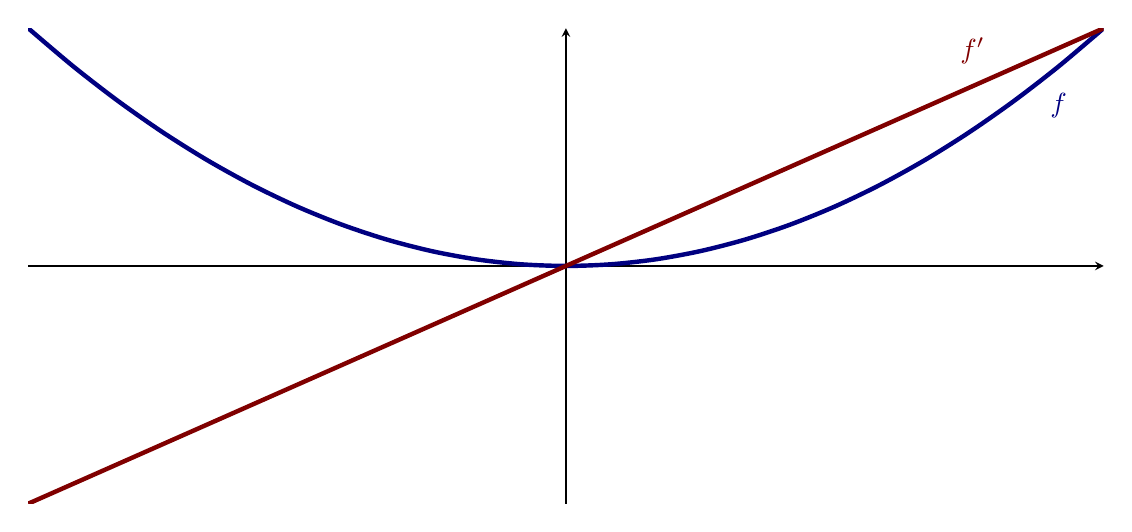
\begin{tikzpicture}
      \begin{axis}[
          xmin=-2,xmax=2,ymin=-4,ymax=4,
          axis lines=center,
          ticks=none,
          width=6in,
          height=3in,
          every axis y label/.style={at=(current axis.above origin),anchor=south},
          every axis x label/.style={at=(current axis.right of origin),anchor=west},
        ]
        %\addplot [ultra thick,dashed, penColor,smooth, domain=(-2:2)] {x^3+.3*x^2-2*x)};
        \addplot [ultra thick,penColor,smooth, domain=(-2:2)] {x^2} node [pos=0.9, below right] {$f$};
        \addplot [ultra thick,penColor2,smooth, domain=(-2:2)] {2*x} node [pos=0.9, above left] {$f'$};
      \end{axis}
    \end{tikzpicture}
  \end{image}

$$f(x)=3x+2, f'(x)=3$$
\begin{image}
    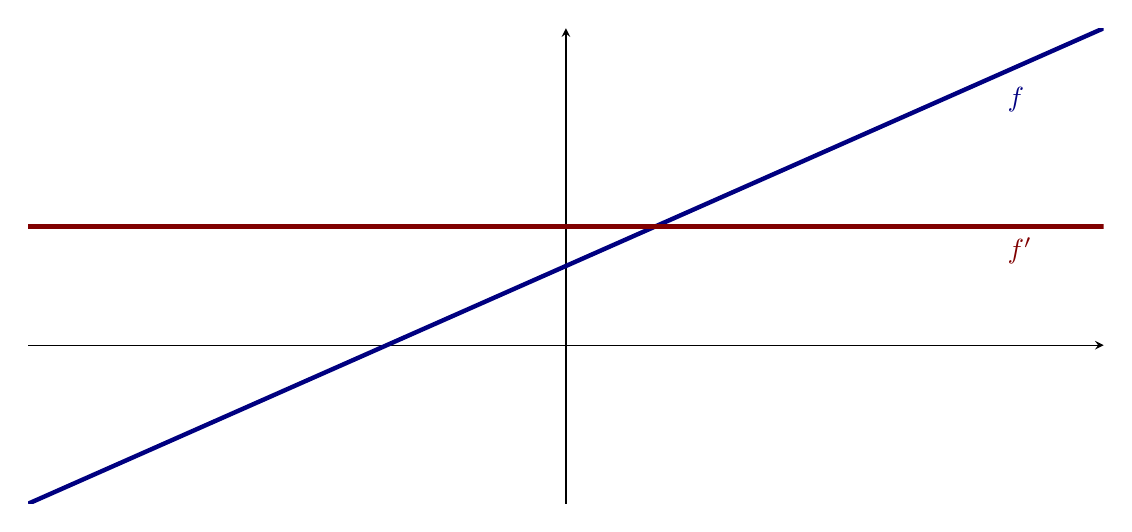
\begin{tikzpicture}
      \begin{axis}[
          xmin=-2,xmax=2,ymin=-4,ymax=8,
          axis lines=center,
          ticks=none,
          width=6in,
          height=3in,
          every axis y label/.style={at=(current axis.above origin),anchor=south},
          every axis x label/.style={at=(current axis.right of origin),anchor=west},
        ]
        %\addplot [ultra thick,dashed, penColor,smooth, domain=(-2:2)] {x^3+.3*x^2-2*x)};
        \addplot [ultra thick,penColor,smooth, domain=(-2:2)] {3*x+2} node [pos=0.9, below right] {$f$};
        \addplot [ultra thick,penColor2,smooth, domain=(-2:2)] {3} node [pos=0.9, below right] {$f'$};

      \end{axis}
    \end{tikzpicture}
  \end{image}

  % (su18:TK) fixed an error below
  % $$f(x)=|x|, f'(x)=\begin{cases} 1 &  \text{for } x<0 \\ -1 &
  %   \text{for } x>0 \end{cases}$$ %fliiped signs
  $$f(x)=|x|, f'(x)=\begin{cases} 1 &  \text{for } x>0 \\ -1 & \text{for } x<0 \end{cases}$$

  \begin{image}
    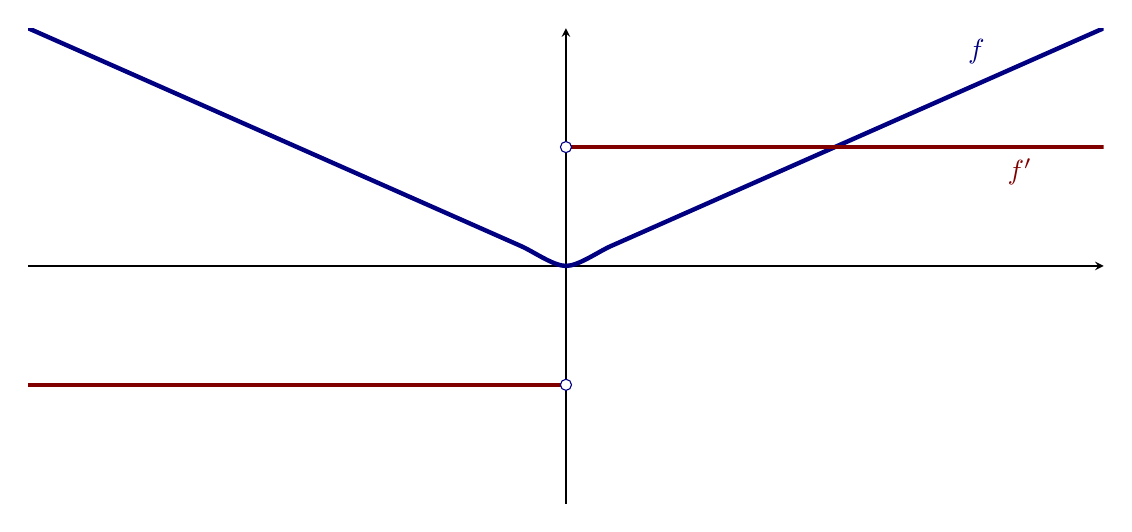
\begin{tikzpicture}
      \begin{axis}[
          xmin=-2,xmax=2,ymin=-2,ymax=2,
          axis lines=center,
          ticks=none,
          width=6in,
          height=3in,
          every axis y label/.style={at=(current axis.above origin),anchor=south},
          every axis x label/.style={at=(current axis.right of origin),anchor=west},
        ]
        %\addplot [ultra thick,dashed, penColor,smooth, domain=(-2:2)] {x^3+.3*x^2-2*x)};
        \addplot [ultra thick,penColor,smooth, domain=(-2:2)] {abs(x)} node [pos=0.9, above left] {$f$};
        \addplot [ultra thick,penColor2,smooth, domain=(-2:0)] {-1};
        \addplot [ultra thick,penColor2,smooth, domain=(0:2)] {1} node [pos=0.8, below right] {$f'$};
        \addplot[color=penColor,fill=background,only marks,mark=*] coordinates{(0,-1)};
        \addplot[color=penColor,fill=background,only marks,mark=*] coordinates{(0,1)};
      \end{axis}
    \end{tikzpicture}
  \end{image}
  \begin{question}
 For each of the three pairs of functions, describe $y=f(x)$ when $f'$
  is positive, and when $f'$  is negative.\\

  \begin{prompt}
    When $f'$ is positive, $y=f(x)$ is \wordChoice{\choice{positive}\choice[correct]{increasing}\choice{negative}\choice{decreasing}}.
    When $f'$ is negative, $y=f(x)$ is \wordChoice{\choice{positive}\choice{increasing}\choice{negative}\choice[correct]{decreasing}}
  \end{prompt}
      \end{question}
\begin{question}
  Here we see the graph of $f'$, the derivative of some function $f$.
  \begin{image}
    \begin{tikzpicture}
      \begin{axis}[
          xmin=-2,xmax=2,ymin=-8,ymax=8,
          axis lines=center,
          ticks=none,
          width=6in,
          height=3in,
          every axis y label/.style={at=(current axis.above origin),anchor=south},
          every axis x label/.style={at=(current axis.right of origin),anchor=west},
        ]
        %\addplot [ultra thick,dashed, penColor,smooth, domain=(-2:2)] {x^3+.3*x^2-2*x)};
        \addplot [ultra thick,penColor,smooth, domain=(-2:2)] {3*x^2+2*.3*x-2)};
      \end{axis}
    \end{tikzpicture}
  \end{image}


    Which of the following graphs could be $y = f(x)$?
     \begin{multipleChoice}
       \choice{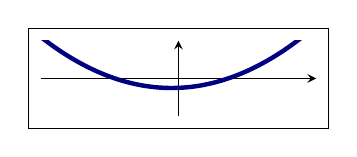
\begin{tikzpicture}[framed,scale=1,baseline=3ex]
           \begin{axis}[
               xmin=-2,xmax=2,ymin=-8,ymax=8,
               axis lines=center,
               ticks=none,
               width=2in,
               height=1in,
               every axis y label/.style={at=(current axis.above origin),anchor=south},
               every axis x label/.style={at=(current axis.right of origin),anchor=west},
             ]
             \addplot [ultra thick,penColor,smooth, domain=(-2:2)] {3*x^2+2*.3*x-2)};
           \end{axis}
       \end{tikzpicture}}
       \choice[correct]{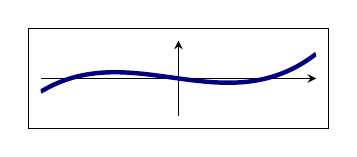
\begin{tikzpicture}[framed,scale=1,baseline=3ex]
           \begin{axis}[
               xmin=-2,xmax=2,ymin=-8,ymax=8,
               axis lines=center,
               ticks=none,
               width=2in,
               height=1in,
               every axis y label/.style={at=(current axis.above origin),anchor=south},
               every axis x label/.style={at=(current axis.right of origin),anchor=west},
             ]
             \addplot [ultra thick,penColor,smooth, domain=(-2:2)] {x^3+.3*x^2-2*x)};
           \end{axis}
       \end{tikzpicture}}
       \choice{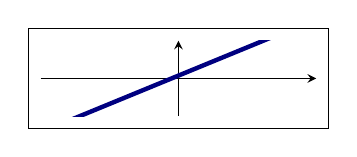
\begin{tikzpicture}[framed,scale=1,baseline=3ex]
           \begin{axis}[
               xmin=-2,xmax=2,ymin=-8,ymax=8,
               axis lines=center,
               ticks=none,
               width=2in,
               height=1in,
               every axis y label/.style={at=(current axis.above origin),anchor=south},
               every axis x label/.style={at=(current axis.right of origin),anchor=west},
             ]
             \addplot [ultra thick,penColor,smooth, domain=(-2:2)] {6*x+2*.3)};
           \end{axis}
       \end{tikzpicture}}
     \end{multipleChoice}

\end{question}


\section{The derivative as a function of functions}

While writing $f'$ is viewing the derivative of $f$ as a function in
its own right, the derivative itself
\[
\ddx
\]
is in fact a function that maps functions to functions,
\begin{align*}
  \ddx x^2 &= 2x\\
  \ddx f(x) &= f'(x).
\end{align*}

\begin{question}
  As a function, is
  \[
  \ddx
  \]
  one-to-one?
  \begin{multipleChoice}
    \choice{yes}
    \choice[correct]{no}
  \end{multipleChoice}
  \begin{feedback}
    Many different functions share the same derivative since the
    derivative records only the slope of the tangent line and not
    the value, or height of the function.
  \end{feedback}
\end{question}

\end{document}

